
\documentclass[]{article}

\usepackage[italian]{babel}
\usepackage[margin=20mm, footskip = 20pt]{geometry}
\usepackage{array}
\usepackage{tabularx}
\usepackage{graphicx}
\usepackage{subfiles}
\usepackage{hyperref}
\usepackage{nameref}
\usepackage{titlesec}
\usepackage{longtable}
\usepackage[table]{xcolor}
\usepackage{titling}
\usepackage{lastpage}
\usepackage{ifthen}
\usepackage{calc}
\usepackage{soulutf8}
\usepackage{contour}
\usepackage{float}
\usepackage{fancyhdr}
\usepackage{multirow}
\usepackage{pgfgantt}
\usepackage{lscape}

\newcommand{\hr}{\par\vspace{-.1\ht\strutbox}\noindent\hrulefill\par}

\graphicspath{ {./}
	{./commons/res}
}

%--------------------------------------------------
% Comandi per inserire contenuto del documento
%--------------------------------------------------
\makeatletter

\newcommand\appendToGraphicsPath[1]{%
	\g@addto@macro\Ginput@path{{#1}}%
}

\newcommand{\setTitle}[1]{%
	\newcommand{\@phTitle}{#1}%
}
\newcommand{\phTitle}{\@phTitle}

\newcommand{\setDate}[1]{%
	\newcommand{\@phDate}{#1}%
}
\newcommand{\phDate}{\@phDate}

\newcommand{\setUso}[1]{%
	\newcommand{\@uso}{#1}%
}
\newcommand{\uso}{\@uso}

\newcommand{\setVersione}[1]{%
	\newcommand{\@versione}{#1}%
}
\newcommand{\versione}{\@versione}

\newcommand{\disabilitaVersione}{%
	\renewcommand{\setVersione}[1]{}%
	\renewcommand{\versione}{DISABILITATA}
}

\newcommand{\setResponsabile}[1]{%
	\newcommand{\@responsabile}{#1}%
}
\newcommand{\responsabile}{\@responsabile}

\newcommand{\setRedattori}[1]{%
	\newcommand{\@redattori}{#1}%
}
\newcommand{\redattori}{\@redattori}

\newcommand{\setVerificatori}[1]{%
	\newcommand{\@verificatori}{#1}%
}
\newcommand{\verificatori}{\@verificatori}

\newcommand{\setModifiche}[1]{%
	\newcommand{\@modifiche}{#1}%
}
\newcommand{\modifiche}{\@modifiche}

\makeatother 

%--------------------------------------------------
% Comandi per i documenti esterni e il glossario
%--------------------------------------------------

\newcommand{\dext}[1]{\textsc{#1\textsubscript{\textit{D}}}}

\newcommand{\glock}[1]{\textsc{#1\textsubscript{\textit{G}}}}

%--------------------------------------------------
% Comandi per impostare sottotitoli di quarto e quinto livello
%--------------------------------------------------

\setcounter{secnumdepth}{4}
\setcounter{tocdepth}{4}

\titleformat{\paragraph}
{\normalfont\normalsize\bfseries}{\theparagraph}{1em}{}
\titlespacing*{\paragraph}{0pt}{2.25ex plus 1ex minus .2ex}{1.5ex plus .2ex}

\titleformat{\subparagraph}
{\normalfont\normalsize\bfseries}{\thesubparagraph}{1em}{}
\titlespacing*{\subparagraph}{0pt}{1.75ex plus 1ex minus .2ex}{.75ex plus .1ex}

\appendToGraphicsPath{../../commons/res/}



%------------------------------
%
% COMANDI DI CONFIGURAZIONE
%
%------------------------------

\setTitle{Manuale utente}

\setVersione{0.0.0}

\setDate{14-07-2021}

\setResponsabile{}

\setRedattori{Valton Tahiraj \\&
}

\setVerificatori{ \\&
}

\setUso{Esterno}

\setModifiche{
	0.0.0 & Valton Tahiraj & Amministratore & 14-07-2021 & Prima stesura
}

\begin{document}

	% Direttive per la creazione del titolo tramite comando maketitle
\title{\huge \textsc{\phTitle{}} \\
	\vspace{11pt} \large \textsc{\phDate{}}}

\author{} % Non toccare
\date{} % Non toccare

%--------------------
% Frontespizio
%--------------------

% Logo del gruppo
\begin{figure}[t!]
	\centering
	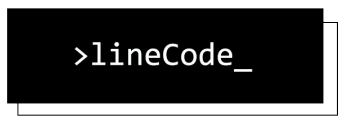
\includegraphics[width=20em]{lclong}
\end{figure}

% Titolo / Nome
\maketitle
\thispagestyle{empty}

% Dati specifici sul doc in forma tabulare
\begin{table}[ht]
	\begin{center}
		\label{tab:Dati sul documento}
		\begin{tabular}{r|l}
			\multicolumn{2}{c}{ \textsc{Dati sul documento} } \\
			\hline
			\textbf{Versione} & \versione{} \\
			\textbf{Uso} & \uso{}  \\
			\textbf{Redattori} & \redattori{} \\
			\textbf{Verificatori} & \verificatori{} \\
			\textbf{Responsabile} & \responsabile{} \\
			\textbf{Destinatari} & lineCode \\
								& prof.\ Vardanega Tullio \\		
								& prof.\ Cardin Riccardo \\
			\ifthenelse{\equal{\uso}{Esterno}}{
								& Sanmarco Informatica
			}{} \\
		\end{tabular}
	\end{center}
\end{table}

\newpage

\renewcommand{\arraystretch}{2} % allarga le righe con dello spazio sotto e sopra
\begin{longtable}[H]{>{\centering\bfseries}m{2cm} >{\centering}m{3.5cm} >{\centering}m{2.5cm} >{\centering}m{3cm} >{\centering\arraybackslash}m{5cm}}
	\rowcolor{lightgray}
	{\textbf{Versione}} & {\textbf{Nominativo}} & {\textbf{Ruolo}} & {\textbf{Data}} & {\textbf{Descrizione}}  \\
	\endfirsthead%
	\rowcolor{lightgray}
	{\textbf{Versione}} & {\textbf{Nominativo}}  & {\textbf{Ruolo}} & {\textbf{Data}} & {\textbf{Descrizione}}  \\
	\endhead%
	\modifiche{}%
\end{longtable}
	\newpage
	\tableofcontents
	\newpage
	\listoffigures
	\listoftables
	\newpage

	%--------------------------------
	%
	% IL CONTENUTO INIZIA DA QUI
	%
	%--------------------------------

	\section{Introduzione}
	\subsection{Scopo del documento}
Il documento ha lo scopo di definire le guidelines del way of working adottato dal team lineCode. Le attività presenti in questo documento sono redatte da processi contenuti nello standard ISO/IEC 12207:1995. Risulta quindi necessario che tutti i membri del gruppo prendano visione di questo documento ai fini di coesione e uniformità all'interno del progetto.

\subsection{Scopo del prodotto}
Il \glock{capitolato} C5 ha come obbiettivo la realizzazione di un applicativo \glock{Real-Time} in grado di guidare delle unità dotate di mobilità autonoma in ambienti specifici, partendo dal presupposto che queste si muovano in ambienti in cui sono presenti altre unità (autonome o meno).

\subsection{Glossario e documenti esterni}
In supporto alla documentazione viene fornito un glossario per chiarire, con una definizione, eventuali termini specifici contenuti in questo documento.
Saranno adottati quindi questi due simboli a pedice:
\begin{itemize}
	\item \textit{D} se indicano un documento specifico;
	\item \textit{G} se incluse nel \dext{glossario}.
\end{itemize}

\subsection{Riferimenti}
	\subsubsection{Riferimenti normativi}
	\begin{itemize}
		\item \textbf{{C5 - PORTACS}}: \url{https://www.math.unipd.it/~tullio/IS-1/2020/Progetto/C5.pdf};
        \item \textbf{Oracle Java Code Conventions}: \url{https://www.oracle.com/technetwork/java/codeconventions-150003.pdf};
        \item \textbf{Angular coding style guide}: \url{https://angular.io/guide/styleguide}.
	\end{itemize}
	\subsubsection{Riferimenti informativi}
	\begin{itemize}
		\item \textbf{ISO/IEC 12207:1995}: \url{https://www.math.unipd.it/~tullio/IS-1/2009/Approfondimenti/ISO_12207-1995.pdf};
		\item \textbf{Gitflow}: \url{http://nvie.com/posts/a-successful-git-branching-model/};
		\item \textbf{Documentazione Zapier}: \url{https://zapier.com/help};
		\item \textbf{Documentazione act}: \url{https://github.com/nektos/act/blob/master/README.md};
		\item \textbf{Studio di Fattibilità}: \dext{Studio di Fattibilità v1.0.0};
		\item \textbf{Piano di Qualifica}: \dext{Piano di Qualifica v2.0.0};
		\item \textbf{Piano di Progetto}: \dext{Piano di Progetto v2.0.0}.
	\end{itemize}
	\newpage
	\section{Requisiti minimi di sistema}
	
	\subsection{Requisiti hardware}
	Non ci sono particolari requisiti hardware, nei dispositivi di test, anche non troppo recenti, non sono stati riscontrati problemi.
	
	\subsection{Requisiti software}
	Il software è stato testato in tutti e tre gli ambienti più utilizzati:
	\begin{itemize}
		\item Linux Ubuntu 19.10;
		\item macOS 14.1;
		\item Windows 10.21H1.
	\end{itemize}  
	
	\newpage
	\section{Installazione}
	\input{res/sez3_installazione.tex}
	\newpage
	\section{Istruzioni per l'utilizzo}
	
\subsection{}
	\newpage


	
	
\end{document}